\documentclass[../report.tex]{subfiles}
\begin{document}
Intel 8086 là bộ vi xử lý 16 bít đầu tiên của Intel và là vi xử lý đầu tiên hỗ trợ tập lệnh
x86. Vi xử lý được sử dụng trong nhiều lĩnh vực khác nhau, nhất là trong các máy IBM PC/XT. Các bộ vi xử lý thuộc họ này vẫn được sử dụng rộng rãi trong một thời gian dài do tính kế thừa của các sản phẩm trong họ x86. Các chương trình viết cho 8086 vẫn có thể chạy
trên các hệ thống tiên tiến sau này.

\subsection{Tập thanh ghi}
\begin{figure}[H]
    \centering
    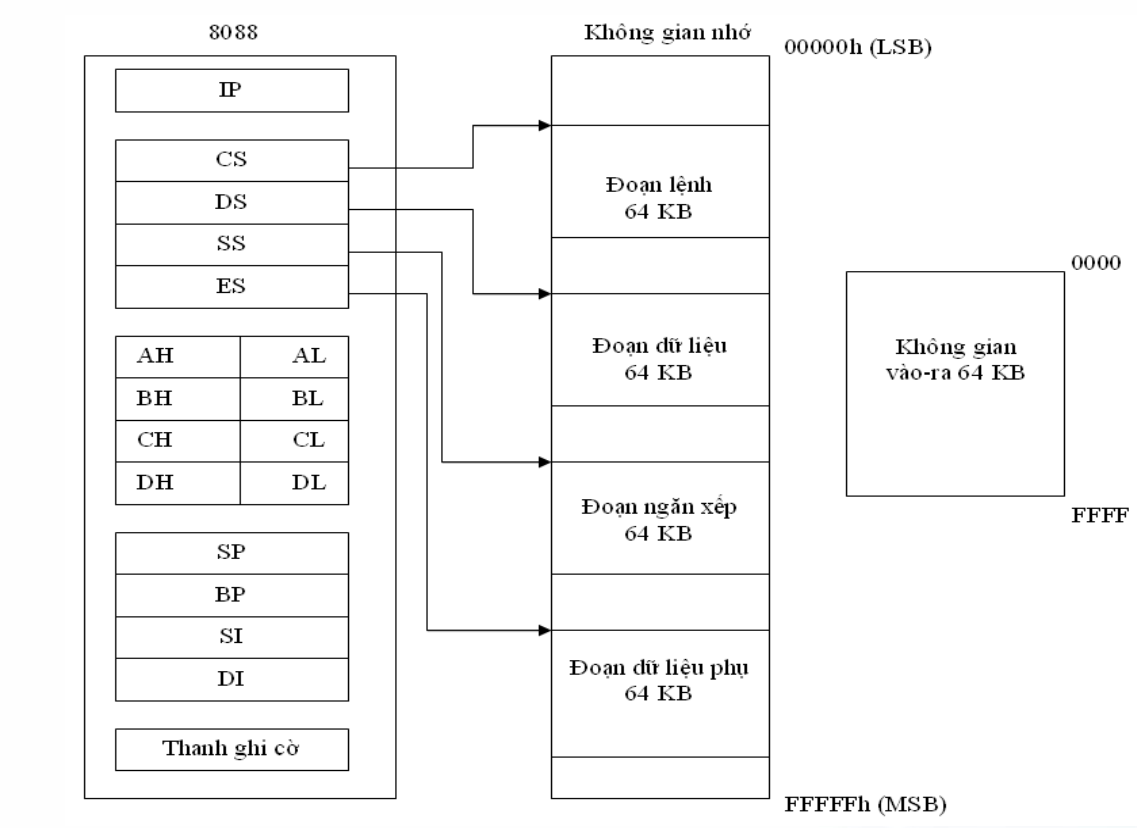
\includegraphics[width=\textwidth]{figures/sw.png}
    \caption{Tập thanh ghi, không gian nhớ và không gian vào ra trong 8086}
\end{figure}
Tập thanh ghi trong 8086 bao gồm:
\begin{itemize}
    \item 4 thanh ghi đoạn:
        \begin{itemize}
            \item CS (Code Segment): thanh ghi đoạn lệnh
            \item DS (Data Segment): thanh ghi đoạn dữ liệu
            \item SS (Stack Segment): thanh ghi đoạn ngăn xếp
            \item ES (Extra Segment): thanh ghi đoạn dữ liệu phụ
        \end{itemize}
        
    \item 3 thanh ghi con trỏ:
    \begin{itemize}
            \item IP: con trỏ lệnh (Instruction Pointer). IP luôn trỏ vào lệnh tiếp theo sẽ được thực hiện
nằm trong đoạn mã CS. Địa chỉ đầy đủ của lệnh tiếp theo có dạng CS:IP
            \item SP: con trỏ ngăn xếp (Stack Pointer). SP luôn trỏ vào đỉnh hiện thời của ngăn xếp nằm
trong đoạn ngăn xếp SS. Địa chỉ đỉnh ngăn xếp có dạng SS:SP
         \item BP: con trỏ cơ sở (Base Pointer). BP luôn trỏ vào một dữ liệu nằm trong đoạn ngăn
xếp SS. Địa chỉ đầy đủ của một phần tử trong đoạn ngăn xếp có dạng SS:BP
    \end{itemize}

    \item 2 thanh ghi chỉ số:
    \begin{itemize}
            \item SI: chỉ số gốc hay nguồn (Source Index). SI chỉ vào dữ liệu trong đoạn dữ liệu DS mà
địa chỉ cụ thể đầy đủ có dạng DS:SI
            \item DI: chỉ số đích (Destination Index). DI chỉ vào dữ liệu trong đoạn dữ liệu DS (hoặc
ES) mà địa chỉ cụ thể đầy đủ có dạng DS:DI (hoặc ES:DI) 
        \end{itemize}
    \item 4 thanh ghi dữ liệu:
    \begin{itemize}
            \item AX (Accumulator): thanh ghi tích lũy. Các kết quả của các thao tác thường được chứa
ở AX (kết quả của phép nhân, chia).
            \item BX (Base): thanh ghi cơ sở, thường dùng để chứa địa chỉ cơ sở của một dãy các ô nhớ. 
            \item CX (Count): thanh đếm. CX thường được dùng để chứa số lần lặp trong trường hợp
các lệnh LOOP (lặp). 
            \item DX (Data): thanh ghi dữ liệu. DX tham gia các thao tác của phép nhân hoặc chia các
số 16 bít. DX thường dùng để chứa địa chỉ của các cổng trong các lệnh vào/ ra dữ liệu.
        \end{itemize}

    \item thanh ghi cờ:
    \begin{figure}[H]
        \centering
        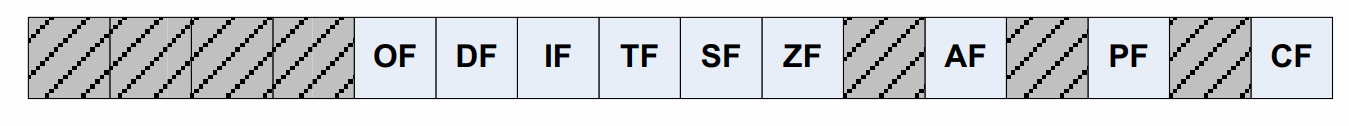
\includegraphics[width=\textwidth]{figures/flag.png}
        \caption{Cấu trúc thanh ghi cờ}
    \end{figure}
        \begin{itemize}
            \item C hoặc CF (Carry Flag): cờ nhớ. CF = 1 khi có nhớ hoặc mượn từ bít có nghĩa lớn
nhất MSB (Most Significant Bit). 
            \item P hoặc PF (Parity Flag): cờ chẵn lẻ. PF phản ánh tính chẵn lẻ của tổng số bít 1 có
trong kết quả. Cờ PF =1 khi tổng số bít 1 trong kết quả là lẻ (odd parity) và PF =0 khi
tổng số bít 1 trong kết quả là chẵn (even parity). 
            \item A hoặc AF (Auxiliary Carry Flag): cờ nhớ phụ rất có ý nghĩa khi ta làm việc với các
số BCD (Binary Coded Decimal). AF = 1 khi có nhớ hoặc mượn từ một số BCD thấp
(4 bít thấp) sang một số BCD cao (4 bít cao). 
            \item Z hoặc ZF (Zero Flag): cờ rỗng. ZF =1 khi kết quả = 0 và ZF = 0 khi kết quả $\neq$ 0.         
            \item S hoặc SF (sign flag): cờ dấu. SF = 1 khi kết quả âm và SF = 0 khi kết quả không âm
            \item O hoặc OF (Overflow Flag): cờ tràn. OF = 1 khi kết quả là một số bù 2 vượt qua ngoài
giới hạn biểu diễn dành cho nó. 
            \item T hoặc TF (Trap Flag): cờ bẫy. TF = 1 thì CPU làm việc ở chế độ chạy từng lệnh (chế
độ này dùng khi cần tìm lỗi trong một chương trình). 
            \item I hoặc IF (Interrupt Enable Flag): cờ cho phép ngắt. IF = 1 thì CPU cho phép các yêu
cầu ngắt (che được) và IF = 0 thì CPU cấm các yêu cầu ngắt. 
            \item D hoặc DF (Direction Flag): cờ hướng. DF = 1 khi CPU làm việc với chuỗi ký tự theo
thứ tự từ phải sang trái, hoặc giảm địa chỉ (vì vậy D chính là cờ lùi) và DF = 0 khi
CPU làm việc với chuỗi ký tự theo thứ tự từ trái sang phải, hoặc tăng địa chỉ .
        \end{itemize}

\end{itemize}

\subsection{Phân đoạn bộ nhớ của 8086}
Do vi xử lý 8086 sử dụng 20 bít địa chỉ để quản lý bộ nhớ trong, như vậy nó có khả
năng phân biệt ra được 220 = 1.048.576 = 1M ô nhớ hay 1Mbyte, vì các bộ nhớ thường tổchức theo byte. Vi xử lí chia không gian 1Mbyte bộ nhớ thành các vùng khác nhau theo nội
dung mà chúng lưu trữ, gồm các vùng nhớ để:
\begin{itemize}
\item Chứa mã chương trình. 
\item Chứa dữ liệu và kết quả của chương trình. 
\item Tạo một vùng nhớ đặc biệt gọi là ngăn xếp (stack) dùng vào việc quản lý các thông số
của bộ vi xử lý khi gọi thự hiện các chương trình con hoặc trở về từ chương trình con. 
\end{itemize}

Để xác định địa chỉ vật lý 20 bít của một ô nhớ nào đó trong một đoạn bất kỳ. CPU 8086 phải dùng
đến 2 thanh ghi 16 bít: một thanh ghi để chứa địa chỉ cơ sở, còn thanh kia chứa độ lệch. Từ
nội dung của cặp thanh ghi đó tạo ra địa chỉ vật lý theo công thức sau: 
\begin{center}
\textbf{Địa chỉ vật lý = Thanh ghi đọan x 10h (16 hệ 10) + Thanh ghi lệch}
\end{center}

Việc dùng 2 thanh ghi để ghi nhớ thông tin về địa chỉ thực chất để tạo ra một loại địa
chỉ gọi là địa chỉ logic và được ký hiệu như sau:

\begin{center}
\textbf{Thanh ghi đoạn: Thanh ghi lệch hay segment: offset}
\end{center}

Địa chỉ kiểu \textbf{segment: offset} là logic vì nó tồn tại dưới dạng giá trị của các thanh ghi cụ
thể bên trông CPU và khi cần thiết truy cập ô nhớ nào đó thì nó phải được đổi ra địa chỉ vật lý
sau đó được đưa lên bus địa chỉ
\newline
\textbf{Ví dụ:}  cặp CS:IP sẽ chỉ ra địa chỉ của lệnh sắp thực hiện trong đoạn mã. Tại một
thời điểm nào đó ta có CS = F000H và IP = FFF0H thì
\begin{center}
Địa chỉ vật lý = F000h x10h + FFF0h = F0000h + FFF0h = FFFF0h
\end{center}
\end{document}